\documentclass[../main.tex]{subfiles}

\begin{document}
\section{Results}\label{sec:results}

\subsection{Simple SIRS model}
In \cref{fig:SIRS_rk4}, the temporal variations of the number of individuals for the three classes ($S$, $I$, $R$) are compared for $b=1$, 2, 3, 4 using the fourth-order Runge-Kutta method. Here, the other parameters are fixed as explained in \cref{sec:populations}. 

\begin{figure}[htb!]
    \centering
    \begin{subfigure}[b]{0.475\textwidth}
    \centering
    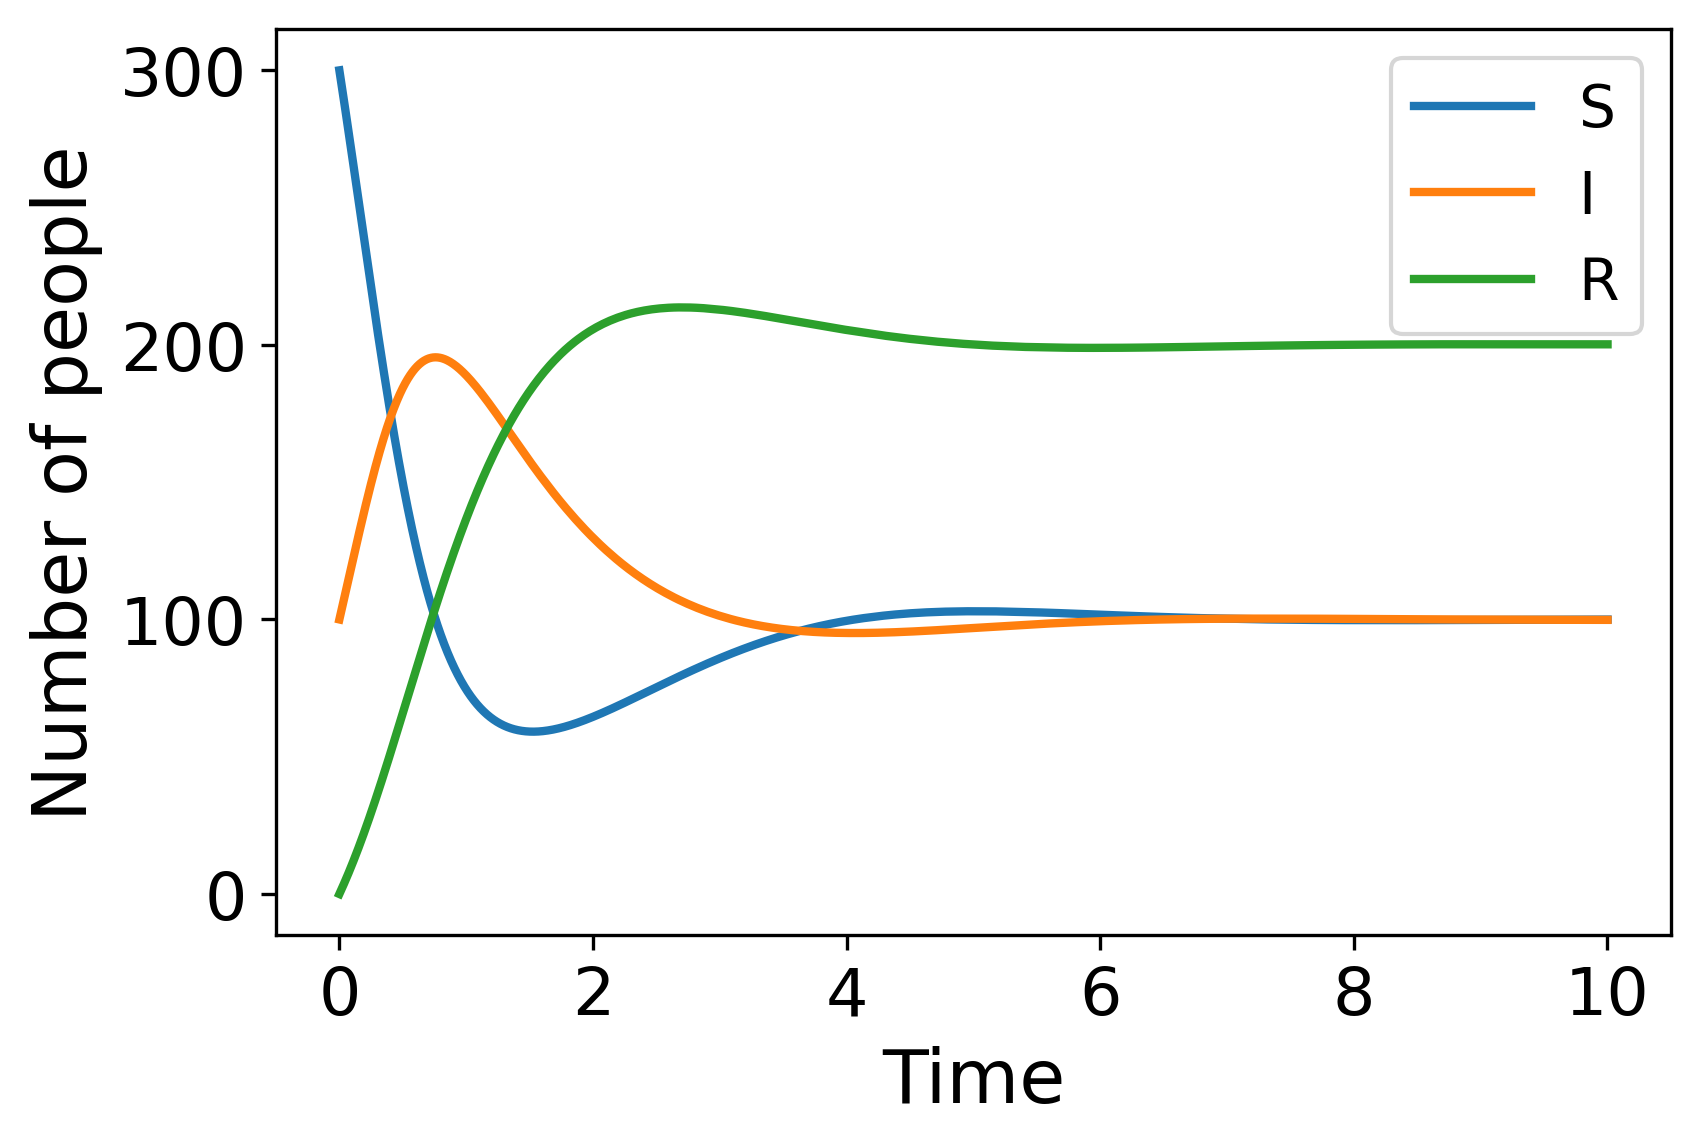
\includegraphics[width=0.9\textwidth]{../figures/SIRS_rk4_b=1.png}
    \caption{}
    \label{fig:b=1}
    \end{subfigure}
    \quad
    \begin{subfigure}[b]{0.475\textwidth}
    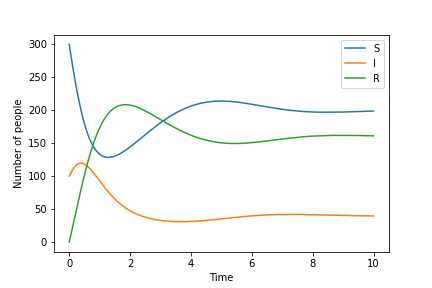
\includegraphics[width=0.9\textwidth]{../figures/SIRS_rk4_b=2.png}
    \caption{}
    \label{fig:b=2}
    \end{subfigure}
    
    \begin{subfigure}[b]{0.475\textwidth}
    \centering
    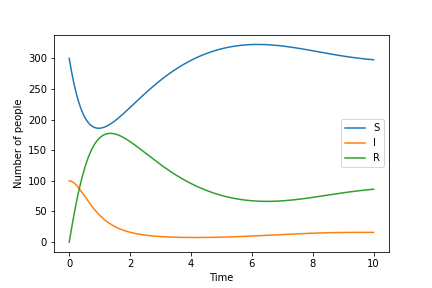
\includegraphics[width=0.9\textwidth]{../figures/SIRS_rk4_b=3.png}
    \caption{}
    \label{fig:b=3}
    \end{subfigure}
    \quad
    \begin{subfigure}[b]{0.475\textwidth}
    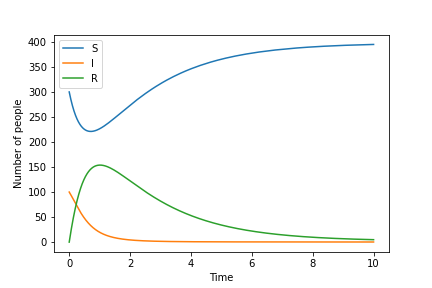
\includegraphics[width=0.9\textwidth]{../figures/SIRS_rk4_b=4.png}
    \caption{}
    \label{fig:b=4}
    \end{subfigure}
    \caption{The numerical solution of the SIRS model using the fourth-order Runge-Kutta method with $N=400$, $I(0)=100$, $a=4$, $c=0.5$ fixed and the comparison of $S$, $I$, $R$ for (a)  $b=1$, (b) $b=2$, (c) $b=3$ and (d) $b=4$.}
    \label{fig:SIRS_rk4}
\end{figure}

For $b=1$, as seen in \cref{fig:b=1}, the number of susceptible individuals decreases with time, reaches a minimum of 59 individuals, gradually increases and reaches an equilibrium at 100 susceptible individuals.
The number of infected individuals increases with time, reaches a peak of 195, gradually decreases and reaches an equilibrium of 100 infected individuals. Meanwhile, the number of recovered individuals increases gradually, has a small dip and reaches an equilibrium at 200 recovered individuals. Next, we look at $b=2$, as seen in \cref{fig:b=2}. Here, the the number of susceptible individuals decreases with time, reaches a minimum of 128 individuals, gradually increases and reaches an equilibrium of 199 susceptible individuals. The number of infected individuals increases for a brief period of  time, reaches a peak of 120, gradually decreases and reaches an equilibrium of 40 infected individuals. While the number of recovered individuals increases gradually, has a small dip and reaches an equilibrium of 161 recovered individuals.
Turning now to  $b=3$, as seen in \cref{fig:b=3}. The number of susceptible individuals gradually decreases with time, reaches a minimum of 185 and approaches 208 with time. The number of infected individuals gradually decreases and approaches 16 with time. The number of recovered individuals increases, reaches a peak of 177 and gradually approaches 86.
Finally, we look at $b=4$ in \cref{fig:b=4}. As expected, the disease does not establish itself in the population. The number of infected individuals gradually decreases and approaches zero with time. While the number of recovered individuals increases, reaches a peak of 154 and gradually approaches zero. 


\subsection{SIRS model with vital dynamics}

\begin{figure}[htb!]
    \centering
    \begin{subfigure}[b]{0.475\textwidth}
    \centering
    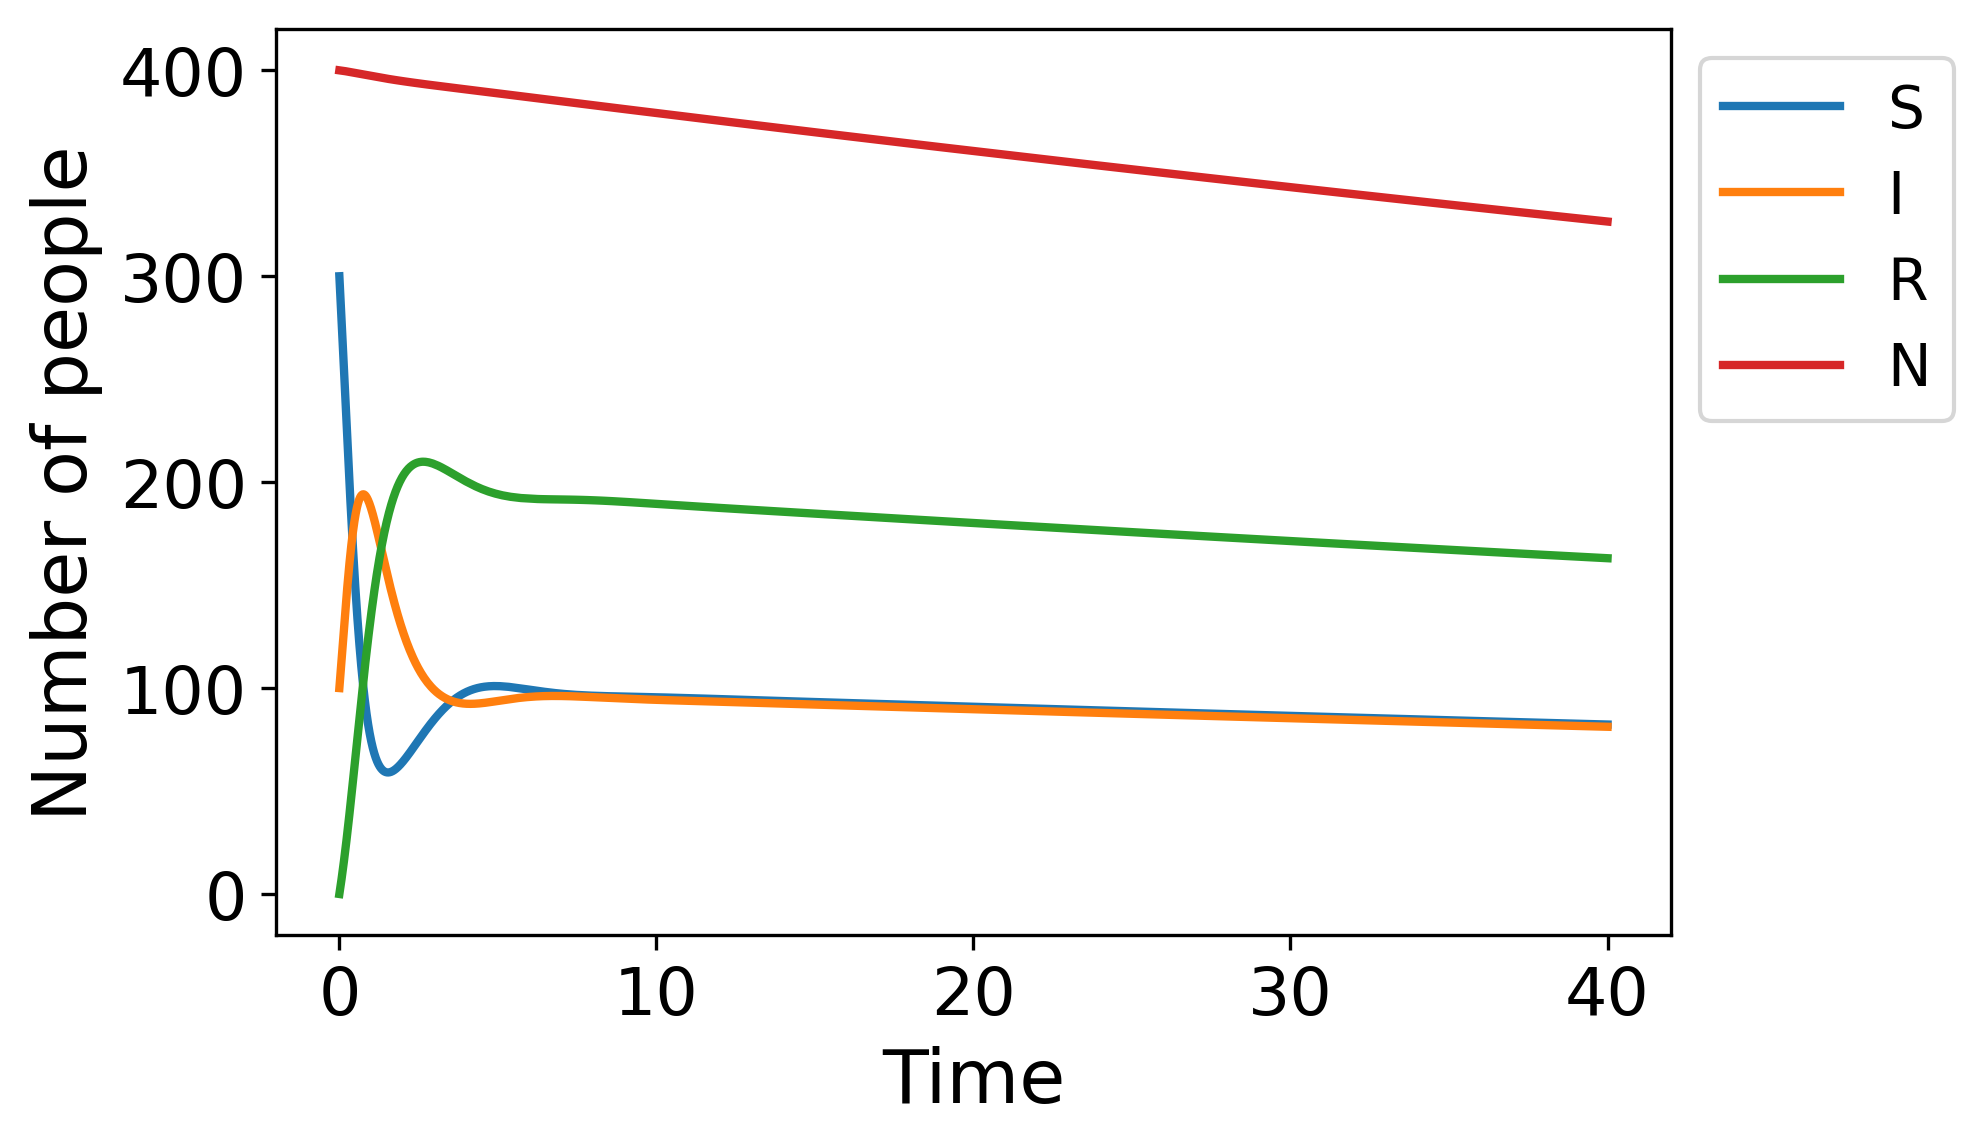
\includegraphics[width=0.9\textwidth]{../figures/SIRS_vital_rk4_b=1.png}
    \caption{}
    \label{fig:vital_b=1}
    \end{subfigure}
    \quad
    \begin{subfigure}[b]{0.475\textwidth}
    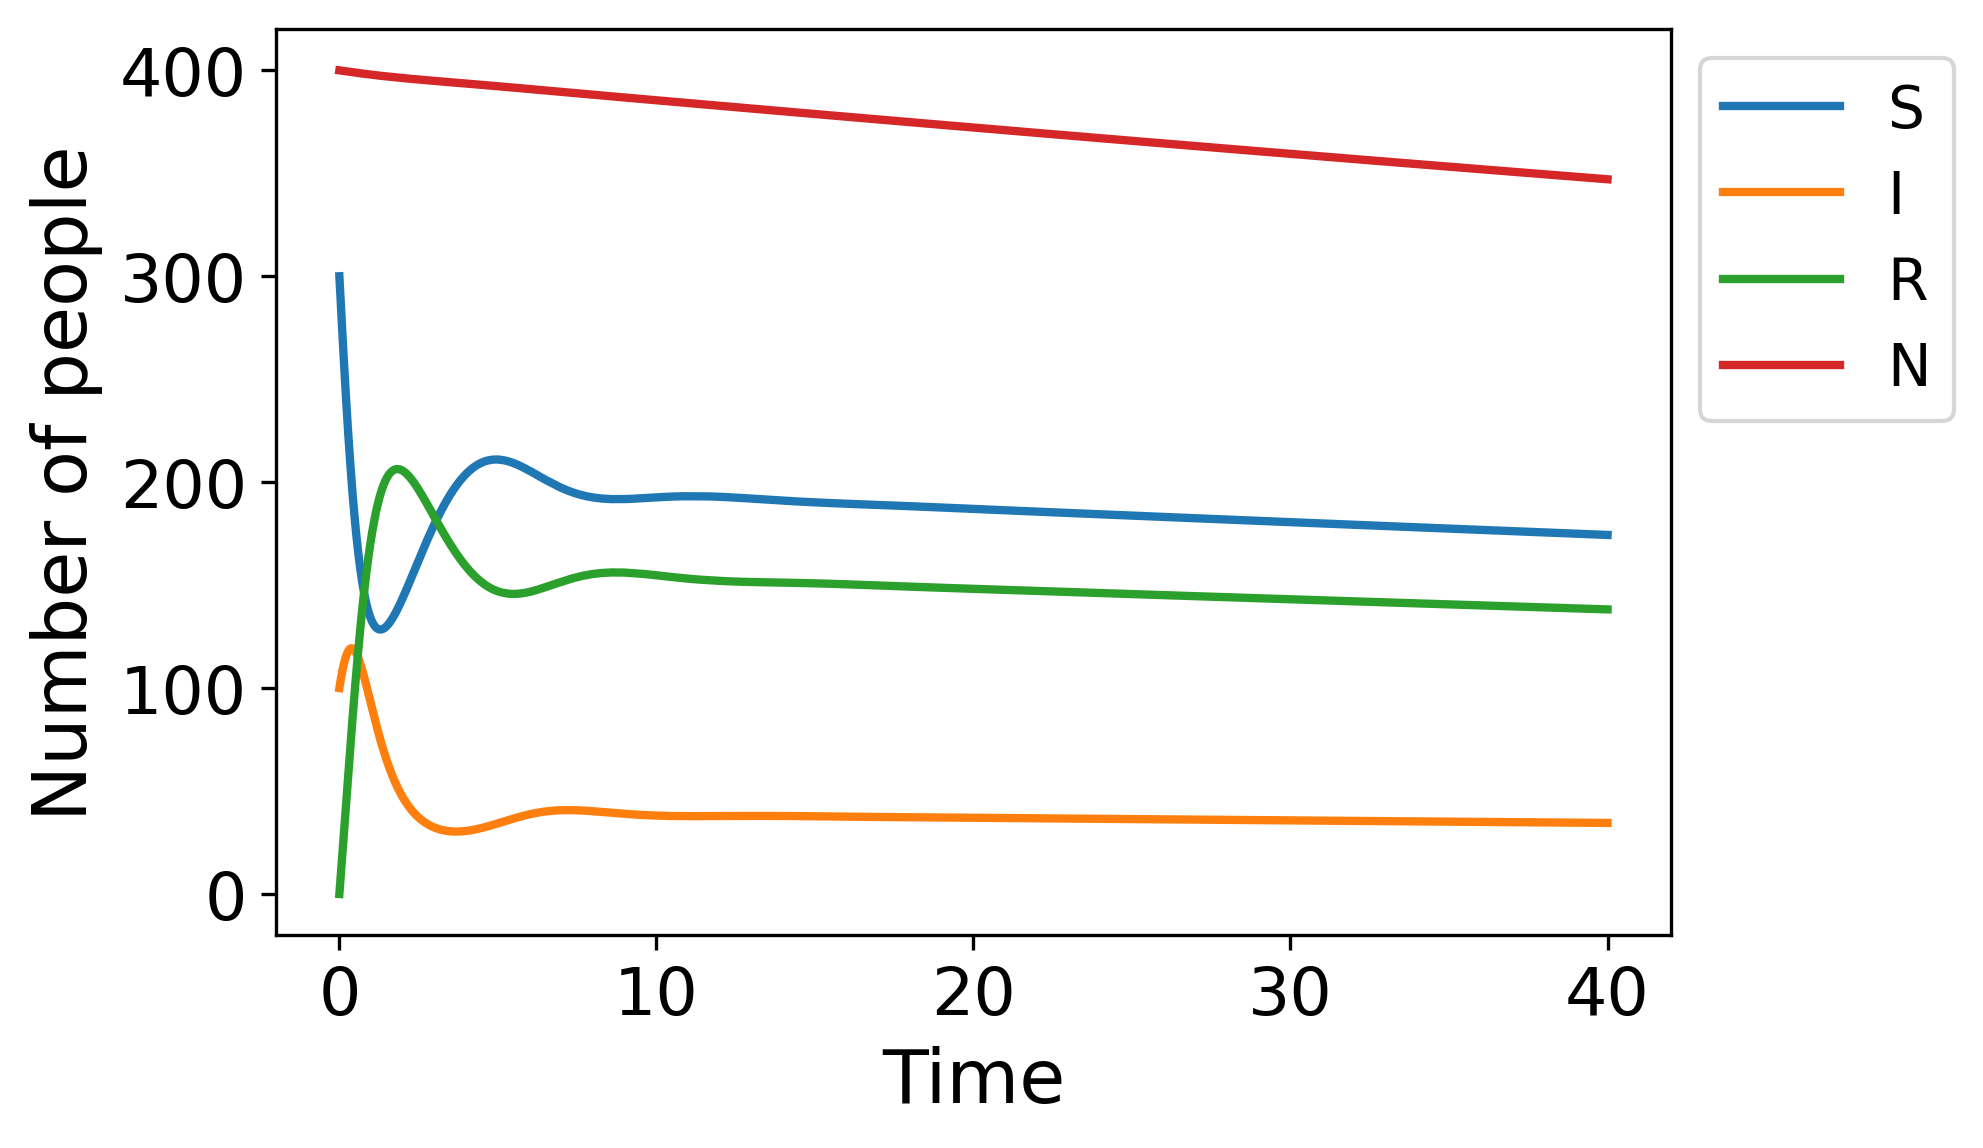
\includegraphics[width=0.9\textwidth]{../figures/SIRS_vital_rk4_b=2.png}
    \caption{}
    \label{fig:vital_b=2}
    \end{subfigure}
    
    \begin{subfigure}[b]{0.475\textwidth}
    \centering
    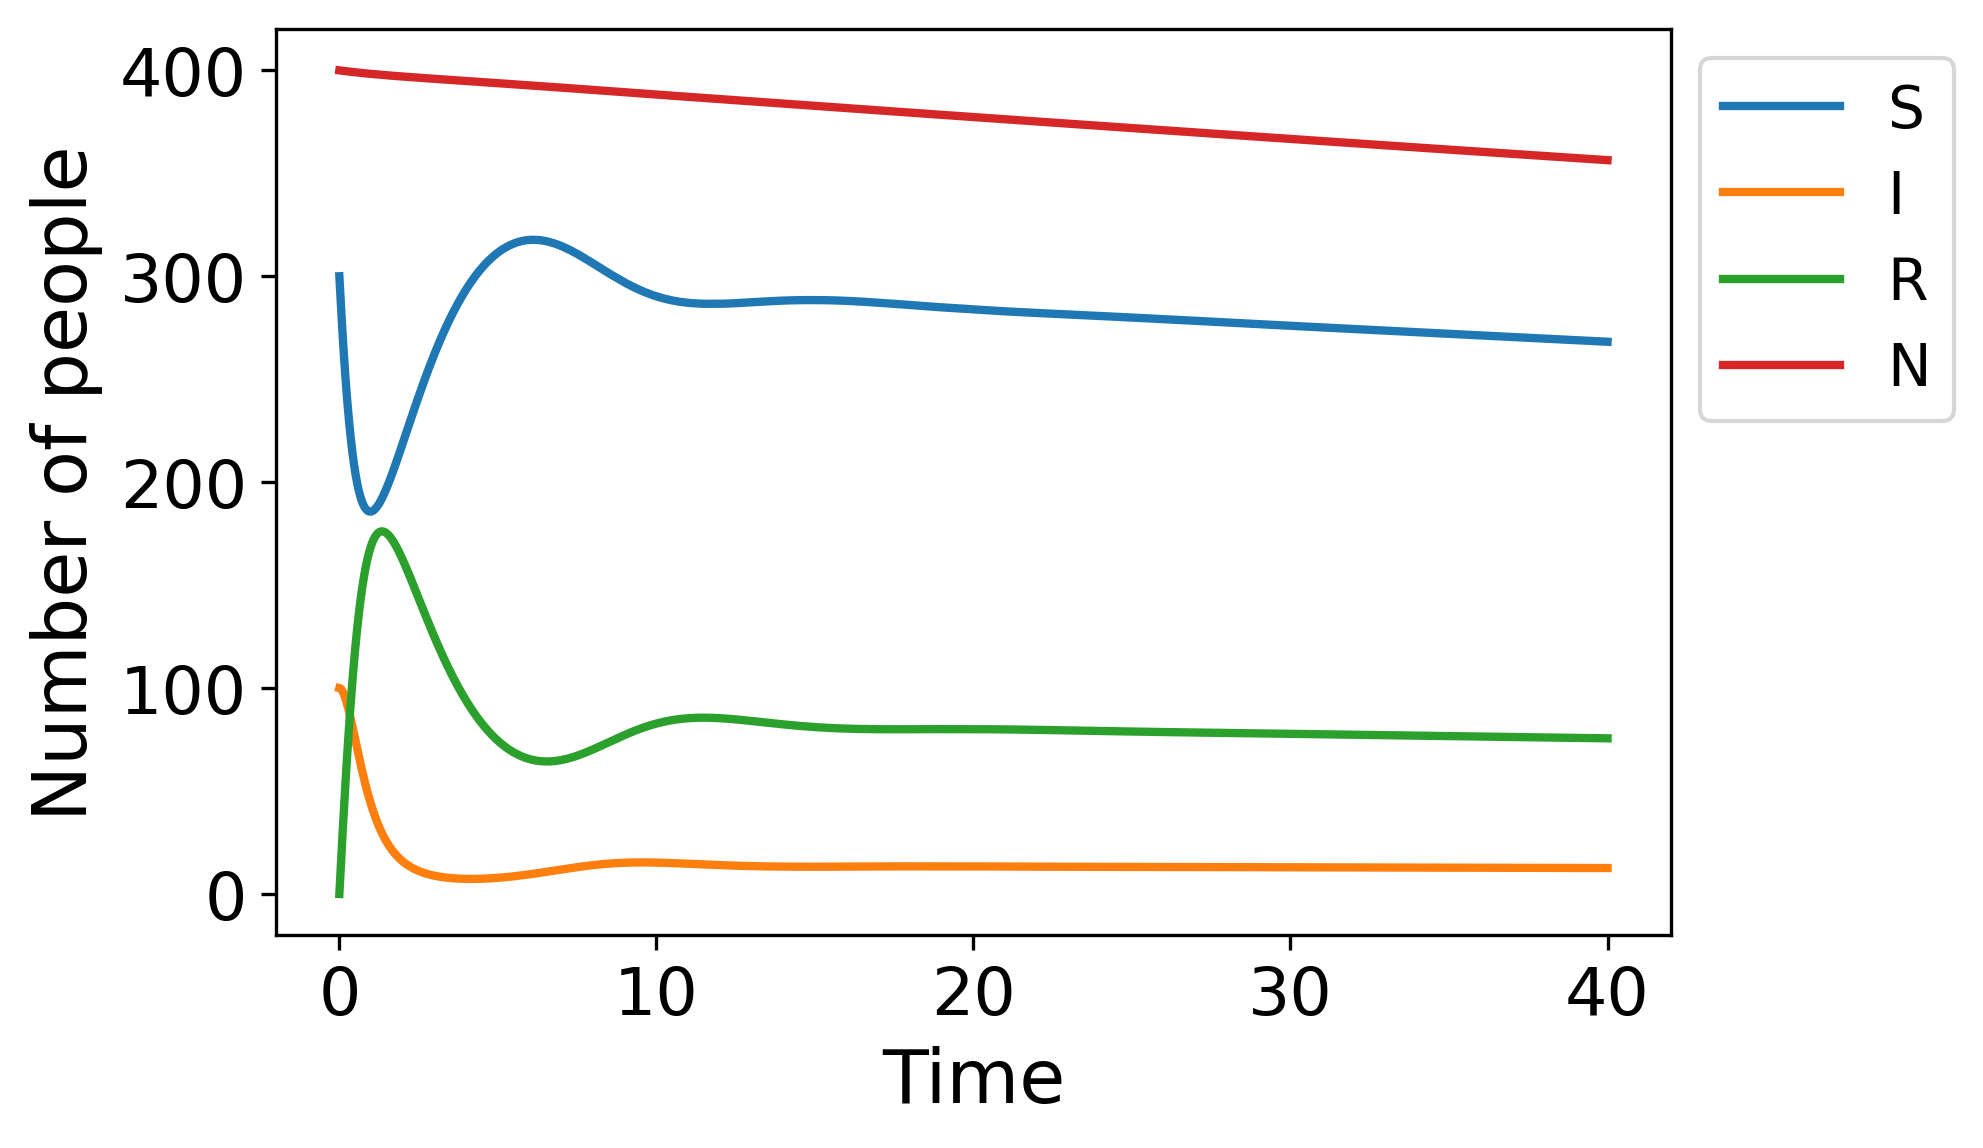
\includegraphics[width=0.9\textwidth]{../figures/SIRS_vital_rk4_b=3.png}
    \caption{}
    \label{fig:vital_b=3}
    \end{subfigure}
    \quad
    \begin{subfigure}[b]{0.475\textwidth}
    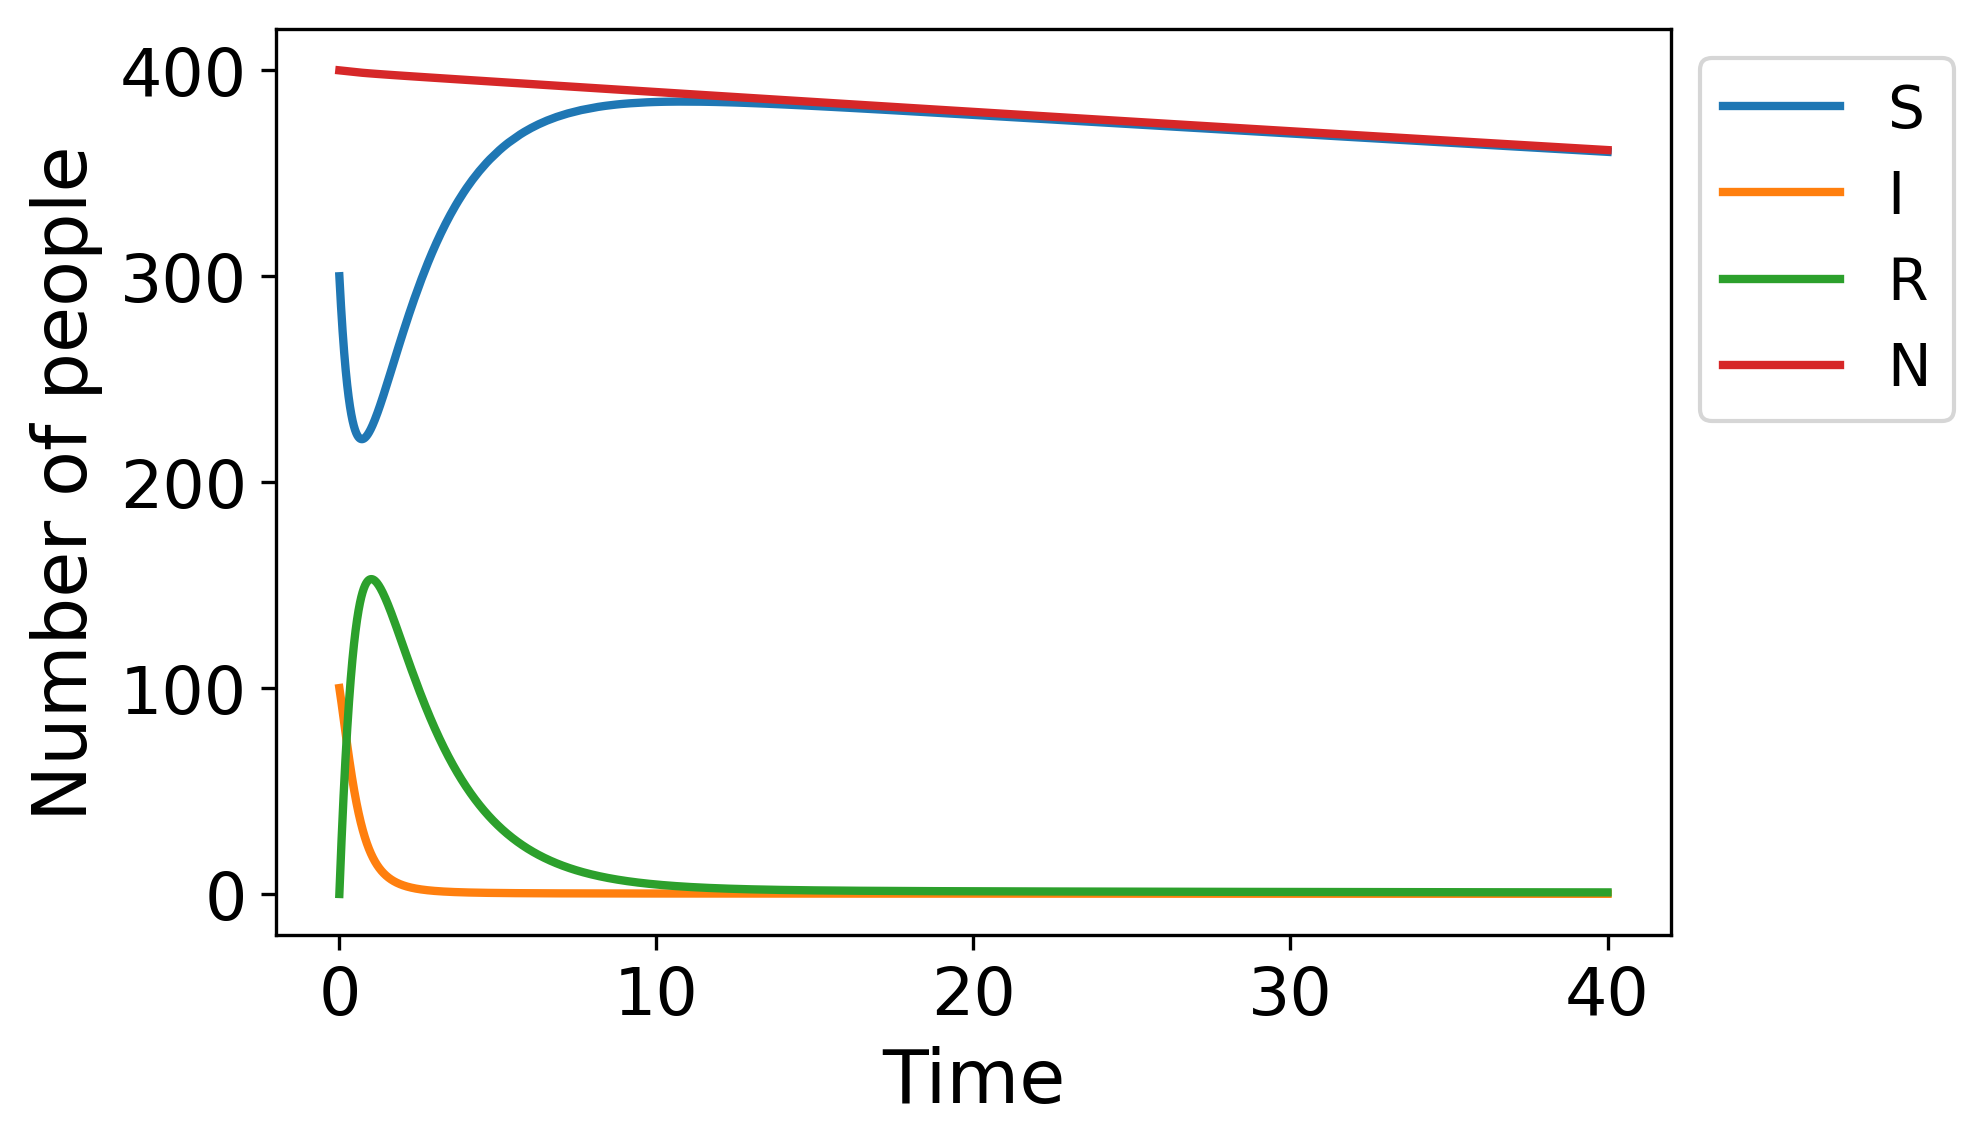
\includegraphics[width=0.9\textwidth]{../figures/SIRS_vital_rk4_b=4.png}
    \caption{}
    \label{fig:vital_b=4}
    \end{subfigure}
    \caption{The numerical solution of the SIRS model with vital dynamics using the fourth-order Runge-Kutta method with $N(0)=400$, $I(0)=100$, $a=4$, $c=0.5$, $d=0.0003$, $d_I=0.01$, $e=0.0005$ fixed and the comparison of $S$, $I$, $R$ for (a)  $b=1$, (b) $b=2$, (c) $b=3$ and (d) $b=4$.}
    \label{fig:SIRS_rk4_vital}
\end{figure}

\subsection{SIRS model with seasonal variation}

\subsection{Vaccination}
\end{document}
